\section{АНАЛІЗ РИНКУ І ПОТОЧНИХ РІШЕНЬ}
На даний момент існує досить багато готових рішень корпоративних порталів. 
Вони можуть забезпечувати підприємства всіма необхідними функціями і додатками, починаючи від системи обліку працівників, і завершуючи системою аналітики та збору даних -- все це залежить від потреб ринку і певної компанії.
Проте майже всі вони здебільшого призначені для великих компаній, і невеличкі компанії або повинні витрачати величезні гроші на купівлю ліцензій, або ж не користуватися усіма перевагами корпоративного порталу.
Тому було проведено загальний огляд продуктів і виділено основні переваги і недоліки, також виділено поточну використовувану ліценцію розповсюдження ПЗ.
\subsection{Переваги та недоліки поточних рішень}
Зробивши аналіз даної сфери, можна виділити декілька основних аспектів, які будуть використані для розробки подальшого програмного продукту.
Левова частка програмного забезпечення корпоративних порталів розроблено згідно стандартів\cite{portlet2}. 
Всі додатки і аплікації можуть без проблем взаємодіяти між собою. 
Проте великою їх нестачею для малої сфери бізнесу є закритість програмного коду і величезна вартість ліцензій.
Тому невеличкі компанії (до 100 людей) просто не мають змоги собі дозволити таку <<розкіш>>.

\subsubsection{Ліцензіювання і відкритість АРІ}
\par Було проведено аналіз поточних продуктів і їх ліцензій, і виявлено, що майже 90\% використовує проприєтарні рішення.
Більш детально розглянуто у таблиці \ref{t:portals}:

{\footnotesize
\begin{longtable}{|c|c|c|}
\captionsetup{justification=centering}
\caption{Список корпоративних порталів і використовувана ліцензія}\label{t:portals}\\
\hline
\multicolumn{1}{|c|}{\textbf{Назва продукту}}&
\multicolumn{1}{c|}{\textbf{Технологія}}&
\multicolumn{1}{c|}{\textbf{Ліцензія}}\\\hline

\endfirsthead
\caption*{\hfill Продовження таблиці \ref{t:portals}}\\\hline

\multicolumn{1}{|c|}{\textbf{Назва продукту}}&
\multicolumn{1}{c|}{\textbf{Технологія}}&
\multicolumn{1}{c|}{\textbf{Ліцензія}}\\\hline
\endhead

 Jetspeed & Java EE & Apache License v2.0\\ \hline
 ATG Portal & Java EE & Proprietary\\ \hline
 Backbase Portal Software & Java EE, .NET & Proprietary \\ \hline 
 Broadvision Portal & Java EE & Proprietary \\ \hline 
 Bluenog ICE & Java EE & Proprietary \\ \hline
 enPortal  & Java EE & Proprietary\\ \hline 
 CommunityManager.NET  & .NET & Proprietary \\ \hline
 eXo Portal & Java EE & Affero General Public License \\ \hline
 eXo Platform & Java EE & Proprietary \\ \hline
 GateIn Portal & Java EE & LGPL \\ \hline
 Hippo CMS & Java EE & Open Source and Proprietary Licenses \\ \hline
 WebSphere Portal & Java EE & Proprietary \\ \hline
 TeamPortal & Java EE & Proprietary \\ \hline
 JBoss Enterprise Portal  & Java EE & LGPL \\ \hline
 IntraNet & ASP.NET & Proprietary \\ \hline
 Liferay Portal & Java EE & Proprietary Licenses \\ \hline
 TeamWox Groupware & C++ & Proprietary \\ \hline
 SharePoint Server & ASP.NET & Proprietary \\ \hline
 Vignette Portal 8.0 & Java EE & Proprietary \\ \hline
 Oracle WebCenter Suite 11g & Java EE & Proprietary \\ \hline
 Oracle WebLogic Portal 10g & Java EE & Proprietary \\ \hline
 Oracle WebCenter Interaction 10g & ASP.NET & Proprietary \\ \hline
 Oracle IAS Portal 10g & Java EE & Proprietary \\ \hline
 Regroup & Ruby & Proprietary \\ \hline
 ACUBE Portal 5.0 & Java EE & Proprietary \\ \hline
 SAP NetWeaver 7.0 & Java EE & Proprietary \\ \hline
 SORCE V9 & ASP.NET & Proprietary \\ \hline
 Sun Java System Portal Server & Java EE & Open Source, licensing \& support plans \\ \hline
 Sun GlassFish Web Space Server  & Java EE & Open Source, licensing \& support plans \\ \hline
 tmsEKP 1.52 & Java EE & Proprietary \\ \hline
 PortalBuilder 5.2 & Java EE & Proprietary \\ \hline
 ProPortal 4.0 & Java EE & Proprietary \\ \hline
 Intrexx & Java EE & Proprietary \\ \hline
 uPortal & Java EE & Apache License v2.0 \\ \hline

\end{longtable}
}


\par Зробивши певний аналіз, можна дійти до висновку, якби невеликим компаніям давати можливість використовувати продукт на підставах вільного розповсюдження коду, то вони б охотніше пробували, і з часом інвестували в нього гроші, або ж просто <<купляли>> підтримку.
Тобто використати одну із відкритих ліцензій типу GNU Public License.
\par Економічна вигода продукту буде базуватися на корпоративній платній підтримці, типу все, починаючи від підбору серверів -- до налаштування і підтримки продукту.
Зате розробники будуть мати змогу додавати свої зміни у загальний репозиторій та виправляти помилки, що значною мірою пришвидшить процес розробки.
Основна стратегія розробки буде націлена на швидкий вихід на ринок і пошук потенційних клієнтів.
Також велика увага буде прикута до ринку пострадянських республік, адже на даний момент ринок бізнесу стрімко розвивається, тобто попит є, а пропозиція не повній мірі відповідає потребі.
Портали, які розробляються, переважно націлені на Європейський та Американський ринок, а також Азію.
Тому, базуючись на цьому, було виділено такі основні вимоги, як врахування нашого законодавства (для прикладу по працевлаштуванню працівників, веденню документації, конвертації валют і тому подібне) та локалізацію сервісу.
Тим більше підтримка користувачів буде набагато легша і ефективніша всередині країни, ніж з-за кордону, що дасть нам перевагу над іншими існуючими продуктами.

\par Також велику увагу буде приділено відкритості АРІ для взаємодії із вже існуючими додатками.
Адже існуючі рішення в основному базуються на закритих протоколах, чим саме змушують користувачів прив'язуватися до їхньої системи і залежати від них.
\par Інтерфейс і система всіх сучасних продуктів дуже <<важкі>> і мульти-функціональні, що потребує затрат значних ресурсів як у користувачів так і на стороні сервера.
Цей аспект також буде максимально спрощений, що в свою чергу дозволить продукту виділитися на ринку малого бізнесу.

\subsection{Технології розробки} 
Базуючись на поточних стандартах \cite{portlet2} та використовуваних базових технологій (таблиця \ref{t:portals}) було прийнято рішення впровадити розробку на базі Java.
Адже саме Sun (зараз Oracle) <<диктує>> моду на ринку стандартизації портлетів, тому буде просто пристосуватися до поточних рішень.
\par Звичайно ж буде використано всі переваги Java EE.
Для гнучкої і швидкої розробки буде застосовано Spring Framework із ORM обгорткою Hibernate поверх бази даних MySQL.
Для фронтенд логіки UI в основному буде використовуватися jQuery фреймворк.
Сервер бекенду буде працювати на Apache Tomcat.
\par На даний момент не планується стандартизація щодо портлетів, просто в майбутньому можливо буде виділено цей пункт для реалізації в системі.

\subsubsection{Мова програмування Java}
\par Java (вимовляється Джава; інколи - Ява) -- об'єктно-орієнтована мова програмування, випущена компанією Sun Microsystems у 1995 році як основний компонент платформи Java. Синтаксис мови багато в чому походить від C та C++. У офіційній реалізації, Java програми компілюються у байткод, який при виконанні інтерпретується віртуальною машиною для конкретної платформи.
\par Sun Microsystems (Oracle) надає компілятор Java та віртуальну машину Java, які задовольняють специфікації Java Community Process, під ліцезією GNU General Public License.
\par Мова значно запозичила синтаксис із C і C++. Зокрема, взято за основу об'єктну модель С++, проте її модифіковано. Усунуто можливість появи деяких конфліктних ситуацій, що могли виникнути через помилки програміста та полегшено сам процес розробки об'єктно-орієнтованих програм. Ряд дій, які в С/C++ повинні здійснювати програмісти, доручено віртуальній машині. Передусім, Java розроблялась як платформо-незалежна мова, тому вона має менше низькорівневих можливостей для роботи з апаратним забезпеченням. За необхідності таких дій java дозволяє викликати підпрограми, написані іншими мовами програмування.

\par Мова програмування Java зародилася в 1991 р. в лабораторіях компанії Sun Microsystems. Розробку проекту започаткував Джеймс Ґослінґ, сам проект мав назву <<Green>>(Зелений). Створення першої робочої версії, яка мала назву <<Oak>>(дуб), зайняло 18 місяців. Оскільки виявилось, що ім'я Oak уже використовувалось іншою фірмою, то в результаті тривалих суперечок навколо назви нової мови з поміж ряду запропонованих було вибрано назву Java, у 1995 р. мову було офіційно перейменовано.
\par Головним мотивом створення Java була потреба в мові програмування, яка б не залежала від платформи (тобто від архітектури) і яку можна було б використовувати для створення програмного забезпечення, яке вбудовується в різноманітні побутові електронні прилади, такі як мобільні засоби зв'язку, пристрої дистанційного керування тощо.
\par Досить скоро майже всі найпопулярніші тогочасні веб-оглядачі отримали можливість запускати <<безпечні>> для системи Java аплети всередині веб-сторінок. У грудні 1998 р. Sun Microsystems випустила Java 2 (спершу під назвою J2SE 1.2), де було реалізовано декілька конфігурацій для різних типів платформ. Наприклад, J2EE призначалася для створення корпоративних застосунків, а значно урізана J2ME для приладів з обмеженими ресурсами, таких як мобільні телефони. У 2006 році в маркетингових цілях, Версії J2 було перейменовано у Java EE, Java ME та Java SE, відповідно.
\par 13 листопада 2006 року Sun випустили більшу частину Java в якості вільного та відкритого програмного забезпечення згідно з умовами GNU General Public License (GPL). 8 травня 2007 корпорація закінчила процес, в результаті якого всі початкові коди Java були випущенні під GPL, за винятком невеликої частини коду, на який Sun не мала авторського права.
\par Період становлення Java збігся у часі з розквітом міжнародної інформаційної служби World Wide Web. Ця обставина відіграла вирішальну роль у майбутньому Java, оскільки Web теж вимагала платформо-незалежних програм. Як наслідок, були зміщені акценти в розробці Sun з побутової електроніки на програмування для Інтернет.

\par Під <<незалежністю від архітектури>> мається на увазі те, що програма, написана на мові Java, працюватиме на будь-якій підтримуваній апаратній чи системній платформі без змін у початковому коді та перекомпіляції.
\par Цього можна досягти, компілюючи початковий Java код у байт-код, який являє собою спрощені машинні команди. Потім програму можна виконати на будь-якій платформі, що має встановлену віртуальну машину Java, яка інтерпретує байткод у код, пристосований до специфіки конкретної операційної системи і процесора. Зараз віртуальні машини Java існують для більшості процесорів і операційних систем.
\par Стандартні бібліотеки забезпечують загальний спосіб доступу до таких платформозалежних особливостей, як обробка графіки, багатопотоковість та роботу з мережами. У деяких версіях задля збільшення продуктивності JVM, байт-код можна компілювати у машинний код до або під час виконання програми.
\par Основна перевага використання байт-коду -- це портативність. Тим не менш, додаткові витрати на інтерпретацію означають, що інтерпретовані програми будуть майже завжди працювати повільніше, ніж скомпільовані у машинний код, і саме тому Java одержала репутацію <<повільної>> мови. Проте, цей розрив суттєво скоротився після введення декількох методів оптимізації у сучасних реалізаціях JVM.
\par Одним із таких методів є англ. just-in-time (JIT) компіляція, що перетворює Java байт-код у машинний під час першого запуску програми, а потім кешує його. У результаті, така програма запускається і виконується швидше, ніж простий інтерпретований код, але ціною додаткових витрат на компіляцію під час виконання. Складніші віртуальні машини також використовують динамічну рекомпіляцію, яка полягає в тому, що віртуальна машина аналізує поведінку запущеної програми й вибірково рекомпілює та оптимізує певні її частини. З використанням динамічної рекомпіляції можна досягти більшого рівня оптимізації, ніж за статичної компіляції, оскільки динамічний компілятор може робити оптимізації на базі знань про довкілля періоду виконання та про завантажені класи. До того ж, він може виявляти так звані гарячі точки (англ. hot spots) -- частини програми, найчастіше внутрішні цикли, які займають найбільше часу при виконанні. JIT компіляція та динамічна рекомпіляція збільшує швидкість Java програм, не втрачаючи при цьому портативності.
\par Існує ще одна технологія оптимізації байткоду, широко відома як статична компіляція, або англ. ahead-of-time (AOT) компіляція. Цей метод передбачає, як і традиційні компілятори, безпосередню компіляцію у машинний код. Це забезпечує хороші показники в порівнянні з інтерпретацією, але за рахунок втрати переносності: скомпільовану таким способом програму можна запустити тільки на одній, цільовій платформі.
\par Швидкість офіційної віртуальної машини Java значно покращилася з моменту випуску ранніх версій, до того ж, деякі випробування показали, що продуктивність JIT компіляторів у порівнянні зі звичайними компіляторами у машинний код майже однакова. Проте ефективність компіляторів не завжди свідчить про швидкість виконання скомпільованого коду, тільки ретельне тестування може виявити справжню ефективність у даній системі.

\par На противагу C++, Java <<об'єктно-орієнтованіша>>. Всі дані і дії групуються в класи об'єктів. Виключенням з повної об'єктності (як скажімо в Smalltalk) є примітивні типи (int, float тощо). Це було свідомим рішенням проектувальників мови задля збільшення швидкості. Через це, Java не вважається повністю об'єктно-орієнтовною мовою.
\par У Java всі об'єкти є похідними від головного об'єкта (він називається просто Object), з якого вони успадковують базову поведінку і властивості.
\par Хоча у C++ вперше стало доступне множинне успадкування, але у Java можливе тільки одинарне успадкування, завдяки чому виключається можливість конфліктів між членами класу(методи і змінні), які успадковуються від базових класів.

\par Java використовує автоматичний збирач сміття для керування пам'яттю під час життєвого циклу об'єкта. Програміст вирішує, коли створювати об'єкти, а віртуальна машина відповідальна за звільнення пам'яті після того, як об'єкт стає непотрібним. Коли до певного об'єкта вже не залишається посилань, збирач сміття може автоматично прибирати його із пам'яті. Проте, витік пам'яті все ж може статися, якщо код, написаний програмістом, має посилання на вже непотрібні об'єкти, наприклад на об'єкти, що зберігаються у діючих контейнерах.
\par Прибирання сміття дозволене у будь-який час. В ідеалі воно відбувається під час бездіяльності програми. Збірка сміття автоматично форсується при нестачі вільної пам'яті в купі для розміщення нового об'єкта, що може призводити до кількасекундного зависання. Тому існують реалізації віртуальної машини Java з прибиральником сміття спеціально створеним для програмування систем реального часу.

\subsubsection{Огляд Java Enterprise Edition, як системи розробки бізнес рішень}
\par Java Platform Enterprise Edition, скорочено Java EE (до версії 5.0 — Java 2 Enterprise Edition або J2EE) -- набір специфікацій і відповідної документації для мови Java, який описує архітектуру серверної платформи для задач середніх і великих підприємств.
\par Специфікації деталізовані настільки, щоб забезпечити переносимість програм з однієї реалізації платформи на іншу. Основна мета специфікацій -- забезпечити масштабованість програми і цілісність даних під час роботи системи. Java EE орієнтована на використання її через веб як в Інтернеті, так і в локальних мережах. Вся специфікація створюється і затверджується через JCP (Java Community Process) в рамках ініціативи Sun Microsystems Inc (тепер Oracle).
\par Java EE є промисловою технологією і в основному використовується в високопродуктивних проектах, в яких є необхідна надійність, масштабованість, гнучкість.
\par Популярності Java EE також сприяє те, що Sun (Oracle) пропонує безкоштовний комплект розробки, SDK, який дозволяє підприємствам розробляти свої системи, не витрачаючи великих коштів. В цей комплект входить сервер програм з ліцензією для розробки.

\subsubsection{Об'єктно-реляційне відображення}
\par ORM (англ. Object-relational mapping, Обє'ктно-реляційна проекція) -- технологія програмування, яка зв'язує бази даних з концепціями об'єктно-орієнтованих мов програмування, створюючи <<віртуальну об'єктну базу даних>>.
\par У об'єктно-орієнтованому програмуванні об'єкти в програмі представляють об'єкти з реального світу. Як приклад можна розглянути адресну книгу, яка містить список людей разом з кількома телефонами і кількома адресами. В термінах об'єктно-орієнтованого програмування вони представлятимуться об'єктами класу <<Людина>>, які міститимуть наступний список полів: ім'я, список (або масив) телефонів і список адрес.
\par Суть проблеми полягає в перетворенні таких об'єктів у форму, в якій вони можуть бути збережені у файлах або базах даних, і які легко можуть бути витягнуті в подальшому, зі збереженням властивостей об'єктів і відносин між ними. Ці об'єкти називають <<постійними>> (англ. persistent). Історично існує кілька підходів до рішення цієї задачі.

\par Вирішення проблеми зберігання даних існує -- це реляційні системи управління базами даних. Використання реляційної бази даних для зберігання об'єктно-орієнтованих даних приводить до семантичного провалу, примушуючи програмістів писати програмне забезпечення, яке повинне уміти як обробляти дані в об'єктно-орієнтованому вигляді, так і вміти зберегти ці дані в реляційній формі. Ця постійна необхідність в перетворенні між двома різними формами даних не тільки сильно знижує продуктивність, але і створює труднощі для програмістів, оскільки обидві форми даних накладають обмеження одна на одну.
\par Реляційні бази даних використовують набір таблиць, що представляють прості дані. Додаткова або зв'язана інформація зберігається в інших таблицях. Часто для зберігання одного об'єкта в реляційній базі даних використовується декілька таблиць -- це, у свою чергу, вимагає застосування операції JOIN для отримання всієї інформації, що відноситься до об'єкта, для її обробки. Наприклад, в розглянутому варіанті із записною книгою, для зберігання даних, швидше за все, використовуватимуться як мінімум дві таблиці: <<люди>> і <<адреси>>, і, можливо, навіть таблиця з телефонними номерами.
\par Оскільки системи управління реляційними базами даних зазвичай не реалізують реляційного представлення фізичного рівня зв'язків, виконання кількох послідовних запитів (що відносяться до однієї <<об'єктно-орієнтованої>> структури даних) може бути дуже витратне. Зокрема, один запит вигляду <<знайти такого-то користувача і всі його телефони і всі його адреси і повернути їх у такому форматі>> швидше за все, буде виконаний швидше за серію запитів вигляду <<Знайти користувача. Знайти його адреси. Знайти його телефони>>. Це відбувається завдяки роботі оптимізатора і витратам на синтаксичний аналіз запиту.
\par Деякі реалізації ORM автоматично синхронізують завантажені в пам'ять об'єкти з базою даних. Для того, щоб це було можливим, після створення SQL-запиту, що перетворює об'єкт в SQL, отримані дані копіюються в поля об'єкта, як у всіх інших реалізаціях ORM. Після цього об'єкт повинен стежити за змінами цих значень і записувати їх у базу даних.
\par Системи управління реляційними базами даних показують хорошу продуктивність на глобальних запитах, які зачіпають велику ділянку бази даних, але об'єктно-орієнтований доступ ефективніший при роботі з малими об'ємами даних, оскільки це дозволяє скоротити семантичний провал між об'єктною і реляційною формами даних.
При одночасному існуванні цих двох різних світів збільшується складність об'єктного коду для роботи з реляційними базами даних, і він стає схильнішим до помилок. Розробники програмного забезпечення, що ґрунтується на базах даних, шукали легший спосіб досягнення постійності їхніх об'єктів.
\par Розроблено безліч пакетів, що знімають необхідність в перетворенні об'єктів для зберігання в реляційних базах даних.
Деякі пакети вирішують цю проблему, надаючи бібліотеки класів, здатних виконувати такі перетворення автоматично. Маючи список таблиць в базі даних і об'єктів в програмі, вони автоматично перетворять запити з одного вигляду в іншій. В результаті запиту об'єкта <<людина>> (з прикладу з адресною книгою) необхідний SQL-запит буде сформований і виконаний, а результати <<магічним>> чином перетворені в об'єкти <<номер телефону>> всередині програми.
\par З погляду програміста система повинна виглядати як постійне сховище об'єктів. Він може просто створювати об'єкти і працювати з ними як завжди, а вони автоматично зберігатимуться в реляційній базі даних.
\par На практиці все не так просто і очевидно. Всі системи ORM зазвичай проявляють себе в тому або іншому вигляді, зменшуючи в деякому роді можливість ігнорування бази даних. Більш того, шар транзакцій може бути повільним і неефективним (особливо в термінах згенерованого SQL). Все це може привести до того, що програми працюватимуть повільніше і використовувати більше пам'яті, чим програми, написані <<вручну>>.
\par Але ORM позбавляє програміста від написання великої кількості коду, часто одноманітного і схильного до помилок, тим самим значно підвищуючи швидкість розробки. Крім того, більшість сучасних реалізацій ORM дозволяють програмістові при необхідності жорстко задати код SQL-запитів, який використовуватиметься при тих або інших діях (збереження в базу даних, завантаження, пошук тощо) з постійним об'єктом.

\subsubsection{jQeury, як система для розробки користувацького інтерфейсу веб-проекту}
\par jQuery -- популярна JavaScript-бібліотека з відкритим програмним кодом. Вона була представлена у січні 2006 року у BarCamp NYC Джоном Ресіґом (John Resig). Використовується більш ніж 31\% від 10,000 найбільш відвідуваних сайтів. jQuery є найпопулярнішою бібліотекою JavaScript, яка потужно використовується на сьогоднішній день\cite{jquery_usage}.
\par jQuery є вільним відкритим програмним забезпеченням з подвійним ліцензуванням під MIT License та GNU General Public License другої версії. Синтаксис jQuery розроблений, щоб зробити орієнтування у навігації зручнішим завдяки вибору елементів DOM, створенню анімації, обробки подій, і розробки AJAX-застосувань. jQuery також надає можливості для розробників, для створення плагінів у верхній частині бібліотеки JavaScript. Використовуючи ці об'єкти, розробники можуть створювати абстракції для низькорівневої взаємодії та створювати анімацію для ефектів високого рівня. Це сприяє створенню потужних і динамічних веб-сторінок.
\par Основне завдання jQuery -- це надавати розробнику легкий та гнучкий інструментарій кросбраузерної адресації DOM об'єктів за допомогою CSS та XPath селекторів. Також даний фреймворк надає інтерфейси для AJAX-застосувань, обробників подій і простої анімації.
Принцип роботи jQuery полягає в використанні класу (функції), який при звертанні до нього повертає сам себе. Таким чином, це дозволяє будувати послідовний ланцюг методів.
\par Бібліотека jQuery є JavaScript файлом, яка включає всю його DOM, події(events), ефекти(effects), і AJAX функції. Вона може бути додана до web-сторінки посиланням на локальну копію, або на одну з копій доступних на публічному сервері (наприклад Google CDN).


\subsubsection{Apache Tomcat -- фронтенд сервер розробки}
\par Apache Tomcat -- контейнер сервлетів, розроблений Apache Software Foundation. Повністю написаний мовою програмування Java та реалізує специфікацію сервлетів і Java Server Pages від Sun Microsystems (Oracle), що є стандартами для розробки веб-застосунків на Java.
\par Члени ASF і незалежні добровольці розвивають та підтримують Tomcat. Користувачі мають вільний доступ до вихідного коду Tomcat за умовами Apache License. Першою релізною версією Tomcat стала версія 3.0.x (попередні версії були випущені Sun для внутрішнього користування).



\subsection{Технічний огляд продукту}
Розглянемо більш детально пункт про наявність сучасних засобів ведення бізнесу. 
Кожна компанія завжди стикається із проблемою ведення обліку працівників, ведення обліку фінансів, спільної роботи над документами та іншим.
Також є величезна і невід'ємна потреба у спільному доступі до документів, до корпоративного календаря, до блогу користувачів, до електронних таблиць та інформаційної дошки.
\par Портал підприємства (також відомий як enterprise information portal (EIP) або корпоративний портал) є основою для інтеграції інформації, людей і процесів в рамках організації. 
Це дає змогу забезпечити єдину точку доступу, часто у вигляді веб-інтерфейсу і призначеної для агрегування та персоналізації інформації за допомогою конкретних програмних додатків. Однією відмінною рисою корпоративних порталів є децентралізоване внесення контенту, управління і збереження на віддаленому сервері та постійне оновлення.


\subsection{Історичний огляд корпоративної сфери}
В середині 1990-х років появилися такі веб-портали як AltaVista, AOL, Excite і Yahoo. 
Вони забезпечували користувачів певним набором функцій (наприклад новини, електронна пошта, погода, котирування акцій і пошук), які часто були представлені у вигляді автономного порталу.
Незабаром підприємства усіх типів і форм почали бачити необхідність аналогічного функціоналу для їх різноманітних потреб, проте із єдиною точкою доступу.
\par До кінця 1990-х років, виробники програмного забезпечення почали розробляти веб-портали для різних підприємств. 
Ці програмні пакети були розроблені таким чином, щоб підприємства могли легко розгортати свої власні налаштування корпоративного порталу та доповнювати його своїми додатками.
Перші постачальники комерційних веб порталів з'явилися в 1998 році, це були такі фірми як: Epicentric, Plumtree  та Viador. 
Ці фірми були основними гравцями на ринку, проте ситуація змінилася в 2002 року, коли на ринок почали виходити постачальники серверних аплікацій, такі як BEA, IBM, Passageways, Oracle Corporation і Sun Microsystems.
Підприємства могли вибрати для своїх цілей декілька порталів, що базувалося на основі їх бізнес-структури та стратегічної спрямованості.
\par У 2003 році розробники Java-порталів випустили стандарт, відомий як JSR-168. 
Він повинен був визначити API для взаємодії між корпоративними порталами та портлетами.
Постачальники програмного забезпечення почали розробляти JSR-168 сумісні портлети, які можуть бути розгорнуті на будь-якому JSR-168 сумісному корпоративному порталі. 
Другий ітераційний стандарт JSR-286 є остаточним на даний момент і випущений 12 червня 2008 року.

\subsection{Портлети, як компоненти веб інтерфейсу}
Портлет -- це змінний компонент інтерфейсу веб-порталу (елемент веб--сторінки), який можливо певним чином підключити до порталу.
Портлет містить в собі фрагменти розмітки, які вбудовуються в сторінку порталу. 
Найчастіше сторінка порталу представляється у вигляді набору портлетів, які взаємодіють між собою. 
Таким чином, портлет (або сукупність портлетів) представляється у вигляді єдиного веб-додатку, розміщеного на порталі. 
Приклади портлетів можуть бути наступними: електронна пошта, повідомлення про погоду, фінансовий стан, останні новини і тому подібне.
Завдяки існуючим стандартам розробники можуть створювати портлети, що легко вбудовуються в будь-який портал, який слідує стандартам і правилам.
\par Існує протокол WSRP, що забезпечує стандарт веб-сервісів і дозволяє автоматично вбудовувати віддалено запущені портлети з різних джерел.
Специфікація Java-портлетів JSR168 дає можливість взаємодіяти між собою портлетам з різних веб-порталів. 
Ця специфікація визначає безліч API для взаємодії контейнерів портлетів і дає різні адреси областей персоналізації, подання та безпеки.
Існує безліч постачальників комерційних контейнерів портлетів. 
Як відомо лідирують у цій галузі IBM, Oracle, Vignette. 
Реалізації від цих постачальників мають додаткові розширення і налаштування, проте деякі із ним можуть бути не затверджені стандартами. 
Крім того, є портали з відкритим вихідним кодом, що підтримують JSR168, такі як корпоративний портал Apache Jetspeed-2 або eXo Portal.
\subsubsection{Огляд системи Apache Pluto}
Розглянемо на прикладі один з найбільш вдалої реалізації стандарту портлетів JSR168 -- це Apache Pluto.
Портлет працює всередині контейнера портлетів (Pluto).
Цей контейнер містить портлет з необхідним середовищем для подальшого виконання.
Контейнер портлетів керує життєвим циклом всіх вікон порталу та надає інтерфейси для портлетів, котрі викликаються всередині нього.
Контейнер також запускає методи на виконання із доступних цільових користувацьких сторінок і взаємодіє із сторінками порталу. Принцип роботи і архітектурні компоненти аплікації Pluto 2.0. зображено на рисунку \ref{pic:pluto}.

    \begin{figure}[!ht]
		\centering
		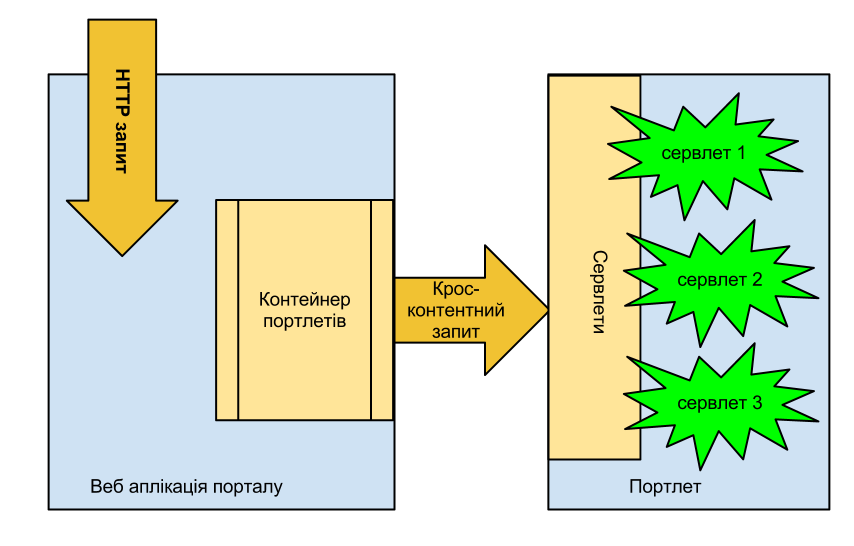
\includegraphics[width=1.00\textwidth]{pluto.png}
		\vspace{6 pt}
		\captionof{figure}{Принцип роботи Apache Pluto}\label{pic:pluto}
	\end{figure}


\par В даному випадку, Pluto вбудований безпосередньо в корпоративний портал. 
Потім через перехресний запит (через веб-додатки) відбувається відправлення запиту для відображення вмісту портлету, який як правило знаходиться в різних додатках на порталі і в контейнерах. 

\subsection{Система керування вмістом}
Система управління контентом (content management system -- CMS) дозволяє публікувати, редагувати і змінювати вміст веб-сторінок, а також обслуговувати портал з центральної сторінки. 
При цьому надається набір процедур, що використовуються для управління робочим процесом у середовищі для спільної роботи.
Вони можуть бути ручні або комп'ютеризовані (в автоматичному режимі).
\subsubsection{Головні функції CMS}
До основних функцій можна віднести наступні пункти:
\begin{itemize}
\item можливість великій кількості людей ділитися інформацією і робити свій вклад в розвиток порталу;
\item контроль доступу до даних на основі ролей користувачів (наприклад визначити роль, яка має тільки права на перегляд інформації, або ж редагування, публікацію тощо);
\item пошук і поширення інформації між користувачами;
\item зменшення дублікацій на вході;
\item спрощене керування корпоративними додатками;
\item відносно легка комунікація між користувачами.
\end{itemize}

\subsubsection{Типи даних та їх використанням}
У CMS дані можуть бути представлені як правило у будь-якій формі: документи, відео, тексти, фотографії, номери телефонів, наукові дані і тому подібне. 
CMS часто використовуються для зберігання, управління, перегляду і публікації документів. 
Також досить поширене використання в якості центрального сховища у зв'язці із централізованою системою контролю версій, що є однією із переваг CMS.
\subsubsection{Управління корпоративною інформацією}
Enterprise Content Management (ECM) -- управління інформаційними ресурсами підприємства або управління корпоративною інформацією.
В даному контексті інформація (контент) передбачається як слабо структурована одиниця -- це можуть бути файли різних форматів, електронні документи з різними наборами полів і т. п.
За визначенням ECM -- це стратегічна інфраструктура і технічна архітектура для підтримки єдиного життєвого циклу неструктурованої інформації різних типів і форматів. 
ECM-системи складаються з додатків, які можуть взаємодіяти між собою, а також використовуватися і продаватися самостійно. 
\par Всі сучасні ECM-системи визначають такі ключові компоненти:
\begin{itemize}
\item управління документами -- довгострокове архівування, автоматизація політик зберігання та відповідності нормам регулюючих органів, забезпечення відповідності законодавчим та галузевим нормам;
\item управління веб-контентом (WCM) -- автоматизація ролі веб-майстра, управління динамічним контентом і взаємодієя між користувачами;
\item  управління мультімедіаконтентом (DAM) -- управління графічними, відео та аудіофайлами, різними маркетинговими матеріалами, наприклад, флеш-банерами, рекламними роликами;
\item управління знаннями (Knowledge Management) -- підтримка систем для накопичення та доставки релевантної для бізнесу інформації;
\item документо-орієнтована взаємодія (співробітництво) -- спільне використання документів користувачами та підтримка проектних команд.
\end{itemize}

\subsection{Система управління документами}
Система управління документами (DMS -- Document management system) -- комп'ютерна система (або набір комп'ютерних програм), що використовується для відстеження та зберігання електронних документів і / або образів (зображень та інших артефактів) паперових документів.
Дане поняття тісно пов'язане з концепцією Content Management System (система керування вмістом) і зазвичай розглядається як компонента Enterprise Content Management System (CMS рівня підприємства).
У загальному випадку системи управління документами надають можливість зберігання, ведення контролю версій, позначення метаданими і безпеку по відношенню до документів, а також індексування і розвинені можливості пошуку документів.
\subsubsection{Інформації про документи у вигляді метаданих}
Метадані зазвичай зберігаються для кожного документа. 
Метадані, наприклад, можуть включати дату занесення документа в сховище і код користувача, котрий виконав зміни до файлу. 
Система управління документами також може витягувати метадані з документа автоматично або запитувати їх у користувача. 
Деякі системи надають сервіс оптичного розпізнавання тексту відсканованих документів, або можливість витягувати текст з електронних документів. 
Використовуючи опрацьований текст система дозволяє здійснювати пошук документа за ключовими словами всередині самого документа.

\subsubsection{Інтеграція документів з іншими системами}
Багато систем управління документами намагаються інтегрувати функцію управління документами безпосередньо в різні додатки, дозволяючи користувачеві отримувати документ відразу зі сховища системи управління документами, робити будь-які модифікації і зберігати його назад в сховище в якості нової версії, і все це проробляти в одному додатку, не виходячи з нього. 
Дана інтеграція в основному доступна для офісних пакетів і поштових клієнтів або для програмного забезпечення призначеного для групової або колективної роботи. 
Інтеграція зазвичай має на увазі використання таких відкритих стандартів як: ODMA, LDAP, WebDAV і SOAP.

\subsubsection{Захоплення тексту та перевід у цифровий формат}
Під захопленням тексту мається на увазі переведення паперових документів в цифровий варіант за допомогою сканерів та багатофункціональних пристроїв.
Також часто використовується програмне забезпечення для оптичного розпізнавання тексту, щоб конвертувати цифрові зображення в текст.

\subsubsection{Індексування документів в єдине сховище даних}
Індексування надає можливість класифікувати документи за допомогою метаданих і індексування словникового тексту, який було витягнутого з документа.
Індексація існує для підтримки розвинених можливостей пошуку документів. 
Одна з головних умов швидкого та якісного пошуку -- це створення індексу документа.

\subsubsection{Призначення сховища даних}
Основне призначення сховища даних -- це для зберігання електронних версій документів. 
Сховище документів також включає в себе і керування тими ж документами, котрі в ньому зберігаються.
Також сховище забезпечує міграцію з одного носія на інший і забезпечує цілісність даних.
Сховище документів може бути як файлове, так і сховище у вигляді СКБД (бази даних). 
У свою чергу, сховище документів в СКБД може бути як в одній базі даних, так і в окремо розподілених базах даних.
        

\subsection{Програмне забезпечення для спільної роботи}
Програмне забезпечення для спільної роботи (англ. collaborative software, groupware, workgroup support systems, group support systems) -- програмне забезпечення створене з метою підтримки взаємодії між людьми, котрі одночасно працюють над вирішенням деяких спільних завдань. 

\subsubsection{Огляд ПЗ для спільної роботи}
Програмне забезпечення для спільної роботи -- це область, яка в значній мірі перекривається з областю CSCW (англ. computer-supported cooperative work (CSCW)).
Часто вважається що ці області еквівалентні, хотя з іншого боку програмне забезпечення для спільної роботи є підчастиною CSCW.
Сюди відносяться такі системи як: електронна пошта, календарі, текстовий чат, Wiki сторінки, корпоративні закладки, блог.
Оскільки ПЗ для спільної роботи відноситься до технологічних елементів CSCW, системи спільної роботи стають корисним аналітичним інструментом у вивченні поведінкових і організаційних параметрів, пов'язаних з більш широкою сферою CSCW.

%FIXME забрати перекладений текст, хтось колись в неті перекладав
\subsubsection{Види взаємодії ПЗ для спільної роботи}
В літературі можна зустріти кілька різних визначень спільної роботи (англ. - collaboration) в застосуванні до інформаційних технологій. Деякі з них виправдані, інші ж настільки великі, що починають втрачати будь-який сенс.
Для того щоб бути впевненим що обрані технології підходять для конкретних потреб, необхідно розуміти відмінності в способах взаємодії людей один з одним.
Є три основні шляхи, по яких здійснюється взаємодія між людьми: 
\begin{itemize}
\item діалог;
\item здійснення угоди;
\item співробітництво.
\end{itemize}

\par Діалог -- це обмін інформацією між одним або кількома учасниками, основна мета якого полягає у з'ясуванні їх позицій і встановлення взаємин. 
Відбувається вільний обмін інформацією без будь-яких обмежень. 
Для підтримання діалогу цілком підходять звичайні комунікаційні технології, такі як телефон, миттєві повідомлення та електронна пошта.
\par Укладення угоди передбачає обмін деякими сутностями і ця процедура зазвичай проводиться за добре визначеними правилами і передбачає зміну відносин між учасниками. Наприклад, один з учасників угоди обмінює гроші на товари і стає покупцем. Новий статус учасників операції та обмінюваних сутностей потрібно зберегти в будь-якому надійному сховищі. Такі операції добре обслуговуються системами управління транзакціями. 
\par Співпраця полягає в тому, що його учасники обмінюються деякими загальними сутностями, на противагу угоді, коли предмет обміну належить лише одному учаснику. 
Як приклад, можна привести просування нової ідеї, створення нової конструкції, досягнення спільних цілей. 
При цьому самі сутності досить розпливчасті і невизначені. 
Таким чином, технології для забезпечення спільної роботи теж повинні бути достатньо гнучкими. 
Вони повинні включати в себе управління документами, ведення обговорень з можливістю сортування за темами, можливість відновити історію внесених змін та багато іншого.
 
\subsubsection{Рівні взаємодії ПЗ під час сумісної роботи}

Рівні взаємодії можна поділити на три категорії по рівню забезпечення взаємодії: засоби зв'язку, засоби для організації конференцій та засоби управління.

\par Електронні засоби зв'язку використовуються для пересилання повідомлень, файлів, даних чи документів між людьми і таким чином дають можливість для обміну інформацією:
\begin{itemize}
\item електронна пошта;
\item факс;
\item голосова пошта;
\item веб-публікації.
\end{itemize}

Електронні конференції також дають змогу для обміну інформацією, проте в інтерактивній формі це є:
\begin{itemize}
\item телефонні конференції;
\item відео і аудіо конференції;
\item Інтернет форуми;
\item чати.
\end{itemize}

Засоби управління діяльності групи:
\begin{itemize}
\item електронні календарі (створення щоденників, системи автоматичного нагадування);
\item системи управління проектами (складання розкладу робіт, відслідковування прогресу виконання);
\item управління документообігом;
\item бази знань: збір, сортування, зберігання і організація доступу до різних форм інформації.
\end{itemize}





\subsection{Інтранет, як підсистема Інтернет}
Інтранет (англ. Intranet, також вживається термін інтрамережа) -- на відміну від мережі Інтернет, це внутрішня приватна мережа організації. 
Як правило, Інтранет -- це Інтернет в <<мініатюрі>>, який побудований на використанні протоколу IP для обміну і спільного використання деякої частини інформації всередині певної організації. 
Це можуть бути списки співробітників, списки телефонів партнерів і замовників. 
Найчастіше під цим терміном мають на увазі тільки видиму частину Інтранет -- внутрішній веб-сайт організації. 
Заснований на базових протоколах HTTP і HTTPS і організований за принципом клієнт-сервер, Інтранет-сайт доступний з будь-якого комп'ютера через браузер. 
\par Таким чином, Інтранет -- це <<приватний>> Інтернет, обмежений віртуальним простором окремо взятої організації. 
Інтранет допускає використання публічних каналів зв'язку, що входять в Інтернет, (VPN), але при цьому забезпечується захист переданих даних і присутній набір заходів щодо припинення проникнення ззовні на корпоративні вузли.
\par Програми в Інтранет засновані на застосуванні Інтернет технологій і особливо веб-технології: гіпертекст у форматі HTML, протокол передачі гіпертексту HTTP і інтерфейс серверних додатків CGI. 
Складовими частинами Інтранет є веб-сервери для статичної або динамічної публікації інформації і браузери для перегляду й інтерпретації гіпертексту.

\subsubsection{Особливості, переваги та недоліки Інтранет}
Інтранет побудований на базі тих же понять і технологій, які використовуються для Інтернету, такі як архітектура клієнт-сервер і стек протоколів Інтернету (TCP / IP). 
В Інтранеті зустрічається все з відомих Інтернет-протоколів, наприклад, протоколи HTTP (веб-служби), SMTP (електронна пошта) і FTP (передача файлів). 
Інтернет-технології часто використовуються для забезпечення сучасними інтерфейсами функцій інформаційних систем, які розміщують корпоративні дані.
\par Інтранет можна представити як приватну версію Інтернету, або як приватнe розширення Інтернету, обмеженого організацією за допомогою брандмауера. 
\par Перші Інтранет веб-сайти і домашні сторінки почали з'являтися в організаціях у 1990-1991 роках. 
Проте за неофіційними даними, термін Інтранет вперше почав використовуватися в 1992 році в таких закладах, як університети і корпорації, що працюють у технічній сфері.
\par Інтранет також протиставляють Екстранет, доступ до Інтранету надано тільки службовцям організації, в той час як до Екстранет можуть отримати доступ клієнти, постачальники, або інші затверджені керівництвом особи. 
В Екстранет-технології крім приватної мережі, користувачі мають доступ до Інтернет ресурсів, але при цьому здійснюються спеціальні заходи для безпечного доступу, авторизації, і аутентифікації.
\par Інтранет компанії не обов'язково повинен забезпечувати доступ до Інтернету. 
Коли такий доступ все ж забезпечується, зазвичай це відбувається через мережевий шлюз з брандмауером, захищаючи Інтранет від несанкціонованого зовнішнього доступу. 
Мережевий шлюз часто також здійснює аутентифікацію користувачів, шифрування даних, і часто -- можливість з'єднання по віртуальній приватній мережі (VPN) що знаходяться за межами підприємства.

Переваги використання Інтранет:
\begin{itemize}
\item висока продуктивність при спільній роботі над деякими загальними проектами;
\item легкий доступ персоналу до даних;
\item гнучкий рівень взаємодії: можна міняти бізнес-схеми взаємодії як по вертикалі, так і по горизонталі;
\item миттєва публікація даних на ресурсах Інтранет дозволяє специфічні корпоративні знання завжди підтримувати у формі і легко отримувати звідусіль в компанії, використовуючи технології мережі та гіпермедіа;
\item дозволяє проводити в життя загальну корпоративну культуру і використовувати гнучкість і універсальність сучасних інформаційних технологій для управління корпоративними роботами.
\end{itemize}


Переваги веб-сайту в Інтранет перед клієнтськими програмами архітектури клієнт-сервер:
\begin{itemize}
\item не потрібно інсталяція програми-клієнта на комп'ютерах користувачів (як неї використовується браузер);
\item відповідно, при змінах функціональності корпоративної інформаційної системи оновлення клієнтського ПЗ також не потрібно;
\item  скорочення тимчасових витрат на рутинних операціях по вводу різних даних, завдяки використанню веб-форм замість обміну даними по електронній пошті;
\item крос-платформна сумісність.% - стандартний браузер на Microsoft Windows, Mac і GNU / Linux / * NIX.
\end{itemize}


Основні недоліки Інтранет:
\begin{itemize}
\item мережа може бути зламана і використана в хакерських цілях;
\item неперевірена або неточна інформація, опублікована в Інтранет, призводить до плутанини і непорозумінь;
\item легкий доступ до корпоративних даних може спровокувати їх витік до конкурентів через несумлінного працівника;
\item працездатність і гнучкість Інтранет вимагають значних накладних витрат на розробку і адміністрування.
\end{itemize}








\subsection{Корпоративна Wiki}

Корпоративна Wiki -- це програмне забезпечення яке призначене для використання в корпоративній сфері і служить особливим чином для підвищення внутрішнього обміну знаннями, з великим акцентом на такі функції, як контроль доступу, інтеграція з іншими програмними продуктами та управління документами. 
\par В організаціях Wiki може або додати або замінити централізовану систему керування контентом. 
Її децентралізований характер дозволяє швидкому поширенню необхідної інформації в межах організації.
Вікі являється швидшим організаційним продуктом ніж централізований репозиторій знань.
Вікі може використовуватися для управління проектами, взаємодією з клієнтами, планування ресурсів підприємства а також інші види управління даними.

\par Особливості Wiki для корпорації включають в себе такі основні аспекти як:
\begin{itemize}
\item швидкий і простий доступ для створення сторінок, які містять посилання на інші корпоративні системи;
\item дозволяє розвантажити електронну пошту за рахунок зберігання всієї необхідної інформації із можливістю спільного доступу людьми які є на даному проекті;
\item гнучка організація інформації;
\item швидкий і розширений пошук.
\end{itemize}



\subsection{Онлайн офіс}
Онлайн офіс -- це набір веб-сервісів у формі програмного забезпечення яке подану кінцевому користувачеві як послуга. 
Набір наданих веб-служб зазвичай включає всі основні можливості традиційних офісних пакетів, такі як текстовий редактор, електронні таблиці, додаток для створення презентацій, органайзер справ і навіть аналоги СКБД. 
Онлайн офіс може бути доступний з будь-якого комп'ютера, у якого є доступ в Інтернет, незалежно від того, яку операційну систему користувач використовує. 
Це дозволяє людям працювати разом по всьому світу і в будь-який час, що веде до створення міжнародних віртуальних команд для спільної роботи над проектами. 


\subsection{Корпоративний блог}
Корпоративний блог -- це блог, що видається організацією і використовується як для зв'язків з громадськістю, так і для внутрішньої організації. 
Або повністю підконтрольний організації, координований і наповнюється нею контентом, але формально з нею не пов'язаний.



\subsubsection{Внутрішньокорпоративний блог}
Внутрішній корпоративний блог -- це важливий засіб комунікації, особливо у великих компаніях. 
Можна навести деякі явні переваги:
\begin{itemize}
\item блог допомагає поліпшити взаємодію співробітників, надає можливості для навчання. Він добре підходить для запуску нових проектів, для роботи в неоднорідних, великих колективах;
\item блог допомагає виявити різні погляди на будь-яке питання. Відкритість для публікації постів і коментарів -- хороша можливість висловитися всім членам колективу;
\item шляхом дискусій на задану тему блог допомагає знайти компроміс при наявності різних точок зору.
Для керівників блог -- можливість налагодити взаємодію зі співробітниками;
\item блог -- це своєрідна <<історія фірми>>, архів ідей і обговорень.
\item найчастіше кожен співробітник може залишити коментар до будь-якого посту. Коло авторів блогу визначається політикою компанії, часто написати пост може будь-який співробітник.
\end{itemize}


Блог має певні переваги перед такими внутрішньокорпоративними комунікаціями, як, наприклад, листування по електронній пошті, зокрема:

\begin{itemize}
\item коли листів стає занадто багато, це ускладнює спілкування;
\item не всі співробітники вміють правильно архівувати листи, в результаті чого вони не зможуть згодом знайти необхідну інформацію.
\end{itemize}

Внутрішній блог -- альтернатива чи доповнення до корпоративних зборів, нарад. 
Співробітники великих компаній часто не мають можливість проводити наради (наприклад, через велику відстань між філіями або зайнятості).

\subsubsection{Публічний блог}
Одна з основних цілей компаній -- це налагодження комунікацій з клієнтами.
% (як поточними, так і потенційними).
Завдяки оперативності публікації постів і можливості коментування публічний корпоративний блог дуже важливий для досягнення цієї мети.
Блоги є цінним доповненням до корпоративного сайту, так як в них може бути представлена альтернативна точка зору на те чи інше питання, ті чи інші продукти компанії можуть бути описані більш простою і доступною мовою.
